\chapter{Conclusions}
\label{Chapter7}
\lhead{Chapter 7. \emph{Conclusions}}

\begin{figure}[H]
  \centering
  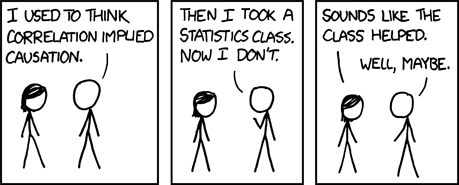
\includegraphics[width=0.6\textwidth]{Figures/xkcd/chapter7.png}
  \caption*{xkcd.com/552}
\end{figure}

In this thesis I have endevoured to demonstrate the possibility of photometrically classifing SLSNe amongst large samples of transients detected by modern, wide-field astronomical surveys. In the process, I have combined our understanding of this class of objects with state-of-the-art Machine Learning and modelling techniques to both define and predict their behaviour in a number of surveys. All this work has been performed with the aim of broadening our understanding of SLSNe as a population. The main results are summerised below.

\section{Modelling SN light curves}
In \cref{Chapter3}, I described the methods for modelling of a variaty of SN and other transients light curves.

\subsection{Modelling SLSNe}
text

\subsection{Modelling CCSN}
text

\subsection{Light Curve interpoaltion using Gaussian Processes}
One of the biggest challenges overcome in this thesis was the problem of interpolating transient light curves. Using Gaussian Process Regression, I developed a method which allowes me to probabilistically inperpolate the data without introducing any models which biases the results or correlates them beyond the standard covariance associated with the uncertainties of the photometric points. This was applied to the light curve of every transient detected by DES as well as all atrificially generated objects in the ML training sample created in \cref{Chapter5}

\section{Rates of SLSN}
text

\subsection{Defining SLSNe}
As the foundation for the work on measuring the rates of SLSNe, I have developed a definition their based on the spin-down of a magnetar model. After fitting the sample of literature SLSNe with the model, I found the objects to concentrate in a small region of the P$_{ms}$-B$_{14}$-$\mathrm{\tau}_M$ parameter space. I have defined this region using an ellipsoid which tightly encapsules all points.

\subsection{Search for SLSN in SNLS}
Using the magnetar model, I fit all SNLS transients and determined that three SN fall within the definition fo a SLSN. Two were the previously discovered, spectroscopically confirmed objects: SNLS06D4eu and SNLS07D2bv. However one object, SNLS07D3bs, was previously unclassified. My modelling suggested a good match to a SLSNe at 0.6$<$z$<1$. Upon this descovery we have uncovered an archival spectrum taken during the life of the transients which shows the redshift to be z=0.74, confirming the object to be consistent with a luminosity of a SLSN.

\subsection{Rate of SLSNe at z$\sim$1}
Bassed on the three SLSN objects detected by SNLS, I performed a Monte Carlo simulation of SNLS to determine the rate of SLSNe and its probaility distribution. I reversed the common approach of weighing each objects by its detection efficiency and observed volume and instead simulated SLSNe and they detectibility starting from a rate informing the number of objects placed in my simulated survey and measuring their detected numbers. I find the rate of SLSNe at z$\sim$1 to be $91^{+76}_{-36}$\,SNe\,Yr$^{-1}$\,Gpc$^{-3}$ or 2.2$^{+1.8}_{-0.9}\times10^{-4}$ of the CCSN rate. This is consistent with other, similar pulications and tentitively demonstrates that the rate of SLSNe follows that of the star formation rate of the universe.

\section{Photometic classification of SN}
text

\subsection{Issues with traditional apprach}
text

\subsection{Training sample}
Using the models of readily available models for SN\,Ia and AGNs, custum build models of SLSNe and CCSN, DES noise models and data augmentation using GPR, I have build a large training sample of SN matching the properties of the the real DES transient sample. Consisting $\sim$300,000 object, this is the largest to date light curve sample used for a photometric classification study and represents objects from the edge of detectibility by DES to local objects.

\subsection{Machine Learning Model}
In order to optimise the classification process, the machine learning models have been divided into two classes. First I worked to create a pure sample of SN-like events in combining the samples of various SN subclasses into a single label classified against the smaple of AGN and spurious survey noise. This produces a classification rate of 99.81\%, as measured on the subsample of the training data, as was further validated using the ground-truth sample of spectroscopically confirmed SLSNe which were all correctly identified in this work.

Upon the identification of a sample of DES SN, consiting of 5273 objects, I attemted to subclassify these objects using only SN light curves as the labeled training set. This again produces a strong classification model, capable of correctly identifying nearly all spectroscopically confirmed SN\,Ia. Applying this to the sample of DES transients I found 500 SLSN candidates, a number which vastly exceeds our expectations based on the rate measured in \cref{Chapter4}. Visual instection of the data showed that the sample is heavily contaminated by SN\,IIP which lacked in our training sample due to the low quality of their available spectral series.

\section{Selecting SLSN}
text

\section{Future Work}
text

\subsection{Expanding the Training Sample}
text

\subsection{Rates of SLSNe from DES}
A natural extention of the work undergone in Chapters \ref{Chapter4}-\ref{Chapter6} is to compute the rate of SLSN using this new and expanded sample of objects. The improvement from 3 to XX objects alone will result in a vastly descred uncertainties in the overall rate of SLSNe. However, more importantly it will be the first ever measurement that will allow for a separation of the rate into separate reshift bins using a homogeneus sample.

....

\subsection{Selecting SLSN in LSST}
text

\subsection{Redshift estimation for photometric SN\,Ia in DES}
Perhaps one of the most interesting results of this thesis, not directly related to its main subject of SLSNe, is the accuracy of photometric selection of SN\,Ia that was obtained purely as a by product of the main analysis. It is worth noting here that the model used for SN\,Ia only included cosmologically
